%% =====================================================================================
%%  Paper B -- Empirical companion (TRIPOD+AI section order)
%%  All tables under tables/ and figures under figures/ are written by the code
%%  (python -m mlmh run ...). Numbers quoted in the text are from results/real/*.csv,
%%  manifests in results/real/*/manifest.json. Compile: pdflatex x2 (no bibtex needed).
%% =====================================================================================
\documentclass[11pt,a4paper]{article}
\usepackage[T1]{fontenc}\usepackage[utf8]{inputenc}\usepackage{lmodern}\usepackage{microtype}
\usepackage[margin=2.4cm]{geometry}\usepackage{booktabs}\usepackage{graphicx}\usepackage{longtable}
\usepackage{amsmath}\usepackage{tabularx}\usepackage{array}\usepackage{ragged2e}\usepackage{xcolor}
\usepackage{rotating}\usepackage{adjustbox}\usepackage[hidelinks]{hyperref}\usepackage{lineno}
\graphicspath{{figures/}}
\newcommand{\todo}[1]{\textcolor{red}{[TODO: #1]}}
\setlength{\parskip}{0.4em}\setlength{\parindent}{0pt}
\title{How much do leaky splits, missing external validation and missing calibration cost?\\
An empirical companion to a PROBAST+AI / TRIPOD+AI appraisal of machine learning for mental-health prediction, on three public actigraphy cohorts}
\author{Aminat Abiola Ajibola$^{1,*}$ \and Roger Nick Anaedevha$^{2}$}
\date{\footnotesize $^{1}$College of Computer Science and Engineering, University of Hafr Al-Batin, Eastern Province, Kingdom of Saudi Arabia \\
$^{2}$Institute of Cyber Intelligence Systems, National Research Nuclear University MEPhI, Moscow, Russian Federation \\[0.3em]
$^{*}$Corresponding author: aajibola@uhb.edu.sa \quad (R.N.A.: roger@robustidps.ai) \\[0.4em]
Code, run manifests and generated tables: \url{https://github.com/rogerpanel/cv/tree/main/mlmh-appraisal}}
\begin{document}
\maketitle
\linenumbers

\begin{abstract}
\textbf{Objective.} A companion systematic review found that machine-learning (ML) models for
mental-health prediction rarely undergo external validation, rarely report calibration, and often
use evaluation designs that leak participant identity. We quantified what each practice costs on
public data. \textbf{Methods.} Three open actigraphy cohorts recorded with the same device:
DEPRESJON (23 depressed, 32 healthy controls), PSYKOSE (22 schizophrenia, the same 32 controls)
and HYPERAKTIV (45 ADHD, 40 clinical controls). One calendar day of minute-level activity was the
analysis unit (1{,}818 unique valid days from 162 participants); 28 statistical and circadian
features fed a majority-class baseline, logistic regression, random forest and XGBoost with
hyper-parameters fixed a priori. E1 compared record-wise with subject-wise five-fold
cross-validation on identical data and seeds. E2 trained on one cohort and evaluated the frozen
model on another, with the shared controls assigned to exactly one cohort. E3 reported Brier score,
calibration slope and intercept, expected calibration error (ECE) and reliability curves for every
model, plus a logistic recalibration arm. Ten seeds; subject-level BCa bootstrap intervals; every
run traceable to a manifest. \textbf{Results.} Record-wise splitting inflated window-level AUROC
by 0.065 (95\% CI 0.024 to 0.122) to 0.114 (0.060 to 0.181) in DEPRESJON, 0.020 (0.006 to 0.041)
to 0.044 (0.017 to 0.080) in PSYKOSE, and 0.130 (0.095 to 0.167) to 0.169 (0.135 to 0.206) in
HYPERAKTIV, where the honest estimate was at chance (0.44 to 0.45) and the leaky one reached 0.60
to 0.65 at subject level. Flexible models inflated more than logistic regression in every cohort.
Transfer from DEPRESJON to PSYKOSE preserved discrimination (AUROC 0.77 to 0.78) but transfer in
the opposite direction reduced AUROC by 0.13 to 0.21, with calibration slopes of 0.27 to 0.63 and
intercepts of 0.7 to 1.4; a label-shift transfer to HYPERAKTIV fell to chance. Under honest
internal validation, slopes were 0.53 to 0.95 and ECE 0.06 to 0.22; recalibration on the training
cohort did not repair the external miscalibration. Subject-level events per candidate predictor
were 0.6 to 0.8. \textbf{Conclusions.} The three practices the review found to be common each
change conclusions on real data, and in the direction of over-optimism. Reporting subject-wise
performance, calibration and subject-level sample sizes should be a condition of publication.
\end{abstract}

\section{Introduction}
Machine-learning models that classify mental-health status from wearable, speech, text or clinical
data are published faster than they are appraised. The companion review \cite{paperA} applied
PROBAST+AI \cite{moons2025} and TRIPOD+AI \cite{collins2024} across the field and counted how
often three practices occur: evaluation designs in which repeated measures from one participant
appear on both sides of a train/test split, absence of any external validation, and absence of any
calibration assessment. Counting is not costing. A reader of the review can still ask whether a
record-wise split matters in practice, whether a model that discriminates well internally will
discriminate at all elsewhere, and whether miscalibration is a real problem for models that are
only ever used to rank.

The published literature on the cohorts used here illustrates the problem. On DEPRESJON the
dataset authors reported a leave-one-patient-out F1 of 0.73 \cite{garciaceja2018}; subsequent
papers report accuracies of 0.85 to 0.96 using day-level or ``modified'' splits
\cite{jmir2025,arxiv2303}; on PSYKOSE, day-level deep models report accuracies near 0.94
\cite{psykose_dl2024}. None reports calibration; none validates across cohorts; and, because the
PSYKOSE control group is the DEPRESJON control group, any paper that uses both cohorts without
noticing has scored half of its test set on training participants.

We designed three experiments, each answering one review outcome, on cohorts chosen so that the
measurement device is constant and only the population changes: (E1) the optimism from
record-wise splitting, measured as a paired difference on identical data; (E2) the loss from
skipping external validation, measured by freezing a model and applying it to another cohort;
(E3) the calibration that would have gone unreported, for every model in E1 and E2. Secondary
analyses report sex-stratified performance (E4) and a transdiagnostic and five-class arm on the
harmonised OBF-Psychiatric release (E5). Our own methods follow TRIPOD+AI item by item
(Supplementary Table S1), because a study that scores others cannot be exempt.

\section{Methods}
\subsection{Source of data and participants}
DEPRESJON \cite{garciaceja2018}, PSYKOSE \cite{jakobsen2020} and HYPERAKTIV \cite{hicks2021} are
open datasets from Haukeland University Hospital and collaborating Norwegian sites, all recorded
with an Actiwatch (Cambridge Neurotechnology) at one-minute resolution, and re-released in
harmonised form as OBF-Psychiatric \cite{obf2025}. DEPRESJON contains 23 in- and outpatients with
unipolar or bipolar depression (MADRS at start of recording, median 24) and 32 healthy controls;
PSYKOSE 22 inpatients with schizophrenia (BPRS median 51) and the same 32 controls; HYPERAKTIV 51
adults with ADHD and 52 clinical controls (psychiatric outpatients without ADHD), of whom 45 and
40 have activity recordings. Recruitment, consent and clinical assessment are described in the
source publications. Table~\ref{tab:cohorts} summarises the analysed participants. Data were
obtained from the dataset authors' download pages and Zenodo; SHA-256 checksums of every file are
recorded in the repository.

\subsection{Outcome}
The outcome was diagnostic group membership: depression versus healthy control (DEPRESJON),
schizophrenia versus healthy control (PSYKOSE), ADHD versus clinical control (HYPERAKTIV). Labels
are participant-level; every window inherits its participant's label, and the data schema rejects a
participant with more than one label.

\subsection{Predictors}
The analysis unit was one calendar day (00:00 to 23:59) of activity counts with at least 80\%
valid minutes; partial first and last days were dropped. Twenty-eight predictors were computed per
day (Supplementary Table S2): distributional statistics (mean, SD, coefficient of variation,
median, 10th and 90th percentiles, maximum, skewness, kurtosis, proportion of zero-count minutes,
mean and SD of $\log(1+x)$), day/night contrasts (08:00 to 22:00 versus night), non-parametric
circadian measures on the hourly profile (M10, L5, relative amplitude, intradaily variability,
sine and cosine of M10 onset), autocorrelation at 5 and 60 minutes, spectral summaries, the
number of rest/activity transitions and the missing-minute fraction. No demographic variable was
used, so that E2 compares populations rather than covariate availability. A raw representation
(the $\log(1+x)$ 1440-minute series) is available for a 1D convolutional network; its results are
reported as a supplementary arm.

\subsection{Sample size}
No sample-size calculation was possible; the cohorts are fixed. We report subject-level events per
candidate predictor (minority-class participants divided by 28) for every training cohort, which
is 0.6 to 0.8, and we report window-level counts alongside, because that is the number most papers
present.

\subsection{Missing data}
Days below the validity threshold were excluded (no participant lost all days). Remaining
missing minutes were ignored in feature computation; missing feature values were imputed with the
training-fold median inside the pipeline.

\subsection{Models and pipeline}
Majority-class baseline, $L_2$-regularised logistic regression ($C=1$, class-balanced), random
forest (500 trees, minimum leaf 2, balanced subsampling) and XGBoost (300 rounds, depth 3, learning
rate 0.05, subsampling 0.8). Hyper-parameters were fixed a priori at library defaults or
conservative values and were not tuned, so that E1 isolates the splitting design. Imputation and
standardisation were fitted on the training fold only inside an \texttt{imblearn} pipeline; no
resampling was applied in the reported runs.

\subsection{Internal validation: E1}
Five-fold cross-validation repeated over ten seeds under two splitters on identical data:
\emph{subject-wise} (stratified group $k$-fold; no participant on both sides of any fold) and
\emph{record-wise} (stratified $k$-fold over days, ignoring participant identity). An automated
test fails the build if any non-E1 configuration requests the record-wise splitter, and the runner
asserts fold disjointness at run time. The inflation is the paired difference (record-wise minus
subject-wise) on the same participants.

\subsection{External validation: E2}
For each ordered pair of cohorts the model was fitted on all windows of cohort A and applied,
frozen, to cohort B. The internal comparator is subject-wise cross-validation on A. Because
DEPRESJON and PSYKOSE share their 32 controls (verified by hashing every participant's activity
series, not by documentation), each shared control was assigned at random (seed 0) to exactly one
cohort, leaving 16 controls on each side; the assignment table is in the repository. The pair
DEPRESJON $\rightarrow$ HYPERAKTIV is a deliberate label-shift test (depression model applied to ADHD
versus clinical controls) and is expected to fail.

\subsection{Performance measures: E3}
Discrimination: AUROC (primary), AUPRC, accuracy, balanced accuracy, macro-F1 and MCC at a 0.5
threshold. Calibration: Brier score, calibration slope (logistic regression of outcome on the
logit of the predicted probability) and intercept (with slope fixed at 1)
\cite{vancalster2019}, ECE with ten equal-width bins, and reliability curves. All measures were
computed at \emph{window} level (the unit most papers report) and at \emph{subject} level (mean
predicted probability per participant). Point estimates are means over seeds; 95\% intervals are
bias-corrected and accelerated bootstrap intervals from 1{,}000 resamples of \emph{participants}
(all of a participant's windows drawn together), with a leave-one-participant-out jackknife for
the acceleration term.

\subsection{Recalibration arm}
For each E2 pair, a logistic recalibration (slope and intercept) was fitted on the training
cohort's out-of-fold predictions and applied to the external predictions, to test whether the
external miscalibration is repairable without access to the target cohort.

\subsection{Fairness: E4}
Subject-wise E1 predictions were stratified by sex (from the harmonised OBF-Psychiatric
metadata) and AUROC, Brier, slope and ECE were recomputed per stratum with subject-level intervals.

\subsection{Open science}
Every run writes a manifest with git commit, configuration hash, seeds, package versions and
dataset checksums; tables and figures in this paper are generated by the code from those runs. The
repository is public under an MIT licence; the data are available from their authors under the
terms cited.

\section{Results}
\subsection{Participants and windows}
% Auto-generated by mlmh.reporting.tables -- do not edit by hand.
\begin{table}[!htbp]
\centering
\caption{Participant characteristics per cohort. HYPERAKTIV controls are psychiatric patients without ADHD (clinical controls); DEPRESJON and PSYKOSE share the same 32 healthy controls. Sex, age band and recording days from the harmonised OBF-Psychiatric metadata; day-windows are the analysis units after the 80\% validity threshold.}
\label{tab:cohorts}
\footnotesize
\begin{adjustbox}{max width=\linewidth}
\begin{tabular}{llrlllrl}
\toprule
Cohort & Group & n & Female, n (\%) & Age (modal band) & Recording days, median (range) & Valid day-windows & Clinical scale, median (IQR) \\
\midrule
depresjon & cases (depression) & 23 & 10 (43) & 45-49 & 13 (5-18) & 405 & MADRS 24 (IQR 18-26) \\
depresjon & controls (healthy\_control) & 32 & 20 (62) & 50-54 & 13 (8-20) & 739 & -- \\
psykose & cases (schizophrenia) & 22 & 3 (14) & 35-39 & 13 (12-14) & 390 & BPRS 51 (IQR 44-58) \\
psykose & controls (healthy\_control) & 32 & 20 (62) & 50-54 & 13 (8-20) & 739 & -- \\
hyperaktiv & cases (adhd) & 45 & 21 (47) & 30-39 & 7 (2-10) & 343 & ASRS 49 (IQR 40-55) \\
hyperaktiv & controls (clinical\_control) & 40 & 20 (50) & 17-29 & 7 (6-10) & 329 & ASRS 34 (IQR 25-43) \\
obf\_psychiatric & cases (adhd, clinical, depression, schizophrenia) & 130 & 54 (42) & 30-39 & 7 (2-18) & 1467 & -- \\
obf\_psychiatric & controls (control) & 32 & 20 (62) & 50-54 & 13 (8-20) & 739 & -- \\
\bottomrule
\end{tabular}
\end{adjustbox}
\end{table}

DEPRESJON yielded 1{,}034 valid days (median 15 per participant), PSYKOSE 1{,}021 (16), HYPERAKTIV
502 (6); no participant was excluded. Series hashing confirmed that the 32 PSYKOSE control
recordings are byte-identical to the 32 DEPRESJON control recordings and that OBF-Psychiatric
contains all 162 participants exactly once.

\subsection{E1: the cost of leaky splitting}
% Auto-generated by mlmh.reporting.tables -- do not edit by hand.
\begin{table}[!htbp]
\centering
\caption{E1, window-level AUROC under subject-wise versus record-wise five-fold cross-validation. Estimates on seed-averaged out-of-fold predictions with subject-level BCa 95\% bootstrap intervals; inflation is the paired record-wise minus subject-wise difference.}
\label{tab:e1}
\footnotesize
\begin{adjustbox}{max width=\linewidth}
\begin{tabular}{llccc}
\toprule
Cohort & Model & AUROC subject-wise & AUROC record-wise & Inflation (paired) \\
\midrule
depresjon & Majority class & 0.465 [0.292, 0.653] & 0.491 [0.459, 0.528] & 0.026 [-0.147, 0.218] \\
depresjon & Logistic regression & 0.779 [0.675, 0.861] & 0.845 [0.781, 0.896] & 0.065 [0.024, 0.122] \\
depresjon & Random forest & 0.770 [0.681, 0.848] & 0.877 [0.823, 0.923] & 0.107 [0.058, 0.168] \\
depresjon & XGBoost & 0.764 [0.675, 0.842] & 0.878 [0.830, 0.918] & 0.114 [0.060, 0.181] \\
psykose & Majority class & 0.437 [0.267, 0.632] & 0.500 [0.470, 0.535] & 0.062 [-0.113, 0.241] \\
psykose & Logistic regression & 0.907 [0.820, 0.942] & 0.927 [0.875, 0.955] & 0.020 [0.006, 0.041] \\
psykose & Random forest & 0.893 [0.798, 0.934] & 0.937 [0.890, 0.962] & 0.044 [0.017, 0.080] \\
psykose & XGBoost & 0.903 [0.810, 0.941] & 0.945 [0.907, 0.969] & 0.042 [0.016, 0.078] \\
hyperaktiv & Majority class & 0.493 [0.355, 0.628] & 0.483 [0.433, 0.533] & -0.010 [-0.170, 0.148] \\
hyperaktiv & Logistic regression & 0.449 [0.360, 0.535] & 0.579 [0.486, 0.661] & 0.130 [0.095, 0.167] \\
hyperaktiv & Random forest & 0.443 [0.361, 0.534] & 0.612 [0.526, 0.692] & 0.169 [0.135, 0.206] \\
hyperaktiv & XGBoost & 0.442 [0.360, 0.524] & 0.593 [0.518, 0.664] & 0.151 [0.116, 0.186] \\
\bottomrule
\end{tabular}
\end{adjustbox}
\end{table}

% Auto-generated by mlmh.reporting.tables -- do not edit by hand.
\begin{table}[!htbp]
\centering
\caption{E1, participant-level AUROC under subject-wise versus record-wise five-fold cross-validation. Estimates on seed-averaged out-of-fold predictions with subject-level BCa 95\% bootstrap intervals; inflation is the paired record-wise minus subject-wise difference.}
\label{tab:e1subj}
\footnotesize
\begin{adjustbox}{max width=\linewidth}
\begin{tabular}{llccc}
\toprule
Cohort & Model & AUROC subject-wise & AUROC record-wise & Inflation (paired) \\
\midrule
depresjon & Majority class & 0.423 [0.300, 0.551] & 0.427 [0.295, 0.555] & 0.001 [-0.191, 0.202] \\
depresjon & Logistic regression & 0.899 [0.822, 0.969] & 0.965 [0.927, 0.990] & 0.065 [0.011, 0.109] \\
depresjon & Random forest & 0.883 [0.812, 0.948] & 0.977 [0.949, 1.000] & 0.094 [0.041, 0.146] \\
depresjon & XGBoost & 0.874 [0.795, 0.947] & 0.985 [0.964, 1.000] & 0.111 [0.040, 0.175] \\
psykose & Majority class & 0.419 [0.278, 0.557] & 0.462 [0.331, 0.593] & 0.043 [-0.148, 0.227] \\
psykose & Logistic regression & 0.974 [0.943, 1.000] & 0.994 [0.983, 1.000] & 0.020 [0.000, 0.043] \\
psykose & Random forest & 0.956 [0.913, 0.997] & 0.994 [0.983, 1.000] & 0.038 [0.000, 0.074] \\
psykose & XGBoost & 0.969 [0.935, 1.000] & 0.997 [0.991, 1.000] & 0.028 [0.000, 0.059] \\
hyperaktiv & Majority class & 0.497 [0.398, 0.597] & 0.443 [0.349, 0.540] & -0.054 [-0.203, 0.106] \\
hyperaktiv & Logistic regression & 0.424 [0.328, 0.519] & 0.601 [0.502, 0.695] & 0.177 [0.131, 0.221] \\
hyperaktiv & Random forest & 0.424 [0.333, 0.518] & 0.641 [0.550, 0.722] & 0.217 [0.177, 0.257] \\
hyperaktiv & XGBoost & 0.438 [0.337, 0.530] & 0.652 [0.555, 0.732] & 0.214 [0.173, 0.261] \\
\bottomrule
\end{tabular}
\end{adjustbox}
\end{table}

% Auto-generated by mlmh.reporting.tables -- do not edit by hand.
\begin{table}[!htbp]
\centering
\caption{E1: window-level discrimination and calibration for every model, cohort and splitting design (per-seed means over ten seeds).}
\label{tab:e1full}
\footnotesize
\begin{adjustbox}{max width=\linewidth}
\begin{tabular}{llllllllll}
\toprule
Cohort & Model & Split & Accuracy & Macro-F1 & AUROC & Brier & Cal. slope & Cal. intercept & ECE \\
\midrule
depresjon & Majority class & subject-wise & 0.653 & 0.395 & 0.482 & 0.227 & -4.01 & -0.00 & 0.000 \\
depresjon & Majority class & record-wise & 0.653 & 0.395 & 0.499 & 0.227 & 0.29 & 0.00 & 0.000 \\
depresjon & Logistic regression & subject-wise & 0.722 & 0.706 & 0.765 & 0.194 & 0.52 & -0.54 & 0.118 \\
depresjon & Logistic regression & record-wise & 0.761 & 0.750 & 0.840 & 0.163 & 0.90 & -0.62 & 0.095 \\
depresjon & Random forest & subject-wise & 0.724 & 0.679 & 0.762 & 0.185 & 0.69 & 0.01 & 0.061 \\
depresjon & Random forest & record-wise & 0.806 & 0.782 & 0.874 & 0.136 & 1.23 & -0.11 & 0.039 \\
depresjon & XGBoost & subject-wise & 0.722 & 0.676 & 0.745 & 0.202 & 0.43 & 0.29 & 0.123 \\
depresjon & XGBoost & record-wise & 0.802 & 0.776 & 0.872 & 0.137 & 0.82 & 0.07 & 0.039 \\
psykose & Majority class & subject-wise & 0.661 & 0.398 & 0.476 & 0.224 & -3.95 & 0.00 & 0.000 \\
psykose & Majority class & record-wise & 0.661 & 0.398 & 0.499 & 0.224 & 0.31 & 0.00 & 0.000 \\
psykose & Logistic regression & subject-wise & 0.856 & 0.842 & 0.906 & 0.115 & 0.90 & -0.60 & 0.086 \\
psykose & Logistic regression & record-wise & 0.868 & 0.855 & 0.926 & 0.103 & 1.07 & -0.62 & 0.078 \\
psykose & Random forest & subject-wise & 0.850 & 0.829 & 0.889 & 0.118 & 0.95 & -0.12 & 0.048 \\
psykose & Random forest & record-wise & 0.878 & 0.861 & 0.936 & 0.093 & 1.32 & -0.17 & 0.048 \\
psykose & XGBoost & subject-wise & 0.862 & 0.842 & 0.899 & 0.108 & 0.71 & 0.15 & 0.046 \\
psykose & XGBoost & record-wise & 0.891 & 0.876 & 0.942 & 0.082 & 0.91 & 0.07 & 0.026 \\
hyperaktiv & Majority class & subject-wise & 0.504 & 0.335 & 0.496 & 0.250 & 0.00 & 0.00 & 0.000 \\
hyperaktiv & Majority class & record-wise & 0.504 & 0.335 & 0.496 & 0.250 & 0.00 & 0.00 & 0.000 \\
hyperaktiv & Logistic regression & subject-wise & 0.461 & 0.460 & 0.463 & 0.286 & -0.21 & -0.01 & 0.160 \\
hyperaktiv & Logistic regression & record-wise & 0.543 & 0.543 & 0.577 & 0.252 & 0.21 & 0.01 & 0.074 \\
hyperaktiv & Random forest & subject-wise & 0.463 & 0.462 & 0.447 & 0.286 & -0.32 & 0.00 & 0.156 \\
hyperaktiv & Random forest & record-wise & 0.571 & 0.571 & 0.603 & 0.245 & 0.57 & 0.00 & 0.055 \\
hyperaktiv & XGBoost & subject-wise & 0.460 & 0.460 & 0.449 & 0.330 & -0.15 & 0.00 & 0.248 \\
hyperaktiv & XGBoost & record-wise & 0.557 & 0.557 & 0.586 & 0.271 & 0.26 & 0.00 & 0.151 \\
\bottomrule
\end{tabular}
\end{adjustbox}
\end{table}

\begin{figure}[!htbp]\centering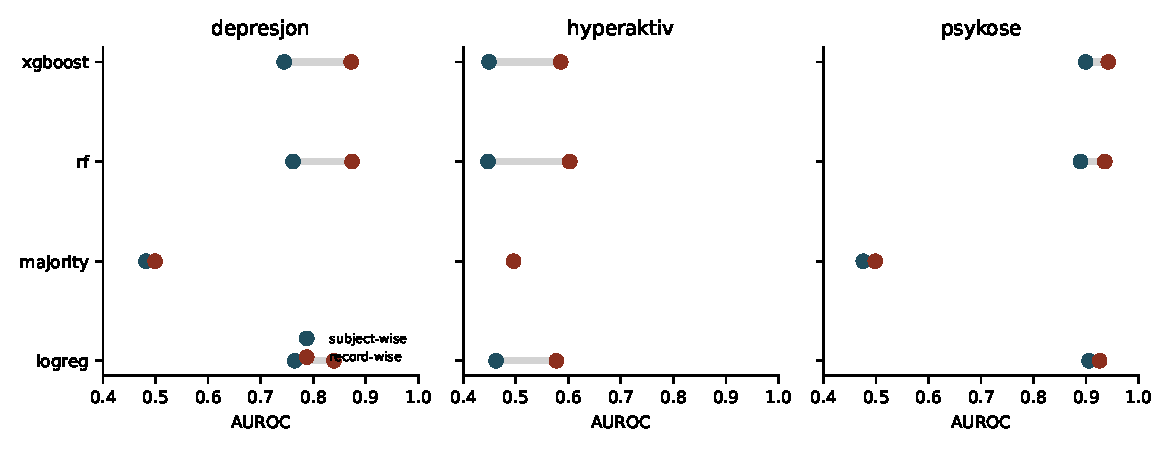
\includegraphics[width=\linewidth]{e1_inflation_auroc.pdf}
\caption{E1. Window-level AUROC of each model under subject-wise (dark) and record-wise (red) five-fold cross-validation, mean over ten seeds. The grey bar is the leakage inflation.}\label{fig:e1}\end{figure}
Record-wise splitting raised window-level AUROC in every cohort and for every informative model
(Table~\ref{tab:e1}, Figure~\ref{fig:e1}; all point estimates below are computed on the
seed-averaged out-of-fold predictions on which the intervals are built, and per-seed means are in
Table~\ref{tab:e1full}). In DEPRESJON, XGBoost rose from 0.764 (95\% CI 0.675 to 0.842) to 0.878
(0.830 to 0.918), a paired inflation of 0.114 (0.060 to 0.181); at subject level the leaky estimate
reached 0.985. In PSYKOSE, where the honest estimate is already high (0.893 to 0.907), the
inflation was 0.020 to 0.044. In HYPERAKTIV the honest estimate was at or below chance for all
three models (0.442 to 0.449 window level; 0.424 to 0.438 subject level), yet record-wise splitting
produced 0.579 to 0.612 at window level and 0.601 to 0.652 at subject level, an inflation of 0.130
to 0.169 with intervals excluding zero. Accuracy and macro-F1 behaved the same
way (Table~\ref{tab:e1full}). Logistic regression inflated least in every cohort (0.065, 0.020,
0.130) and the tree ensembles most.

\subsection{E2: the cost of skipping external validation}
% Auto-generated by mlmh -- do not edit by hand.
\begin{table}[!htbp]
\centering
\caption{E2: internal (subject-wise CV on the training cohort) versus external (unchanged model applied to the second cohort) performance. Window-level estimates, mean over seeds, subject-level BCa 95\% intervals. EPV = minority-class subjects per candidate predictor in the training cohort.}
\label{tab:e2}
\footnotesize
\begin{adjustbox}{max width=\linewidth}
\begin{tabular}{llllllllll}
\toprule
Train $\rightarrow$ Test & Model & EPV & Internal AUROC & External AUROC & $\Delta$ & Int. slope & Ext. slope & Ext. intercept & Ext. Brier \\
\midrule
depresjon $\rightarrow$ psykose & Majority class & 0.6 & 0.465 [0.224, 0.662] & 0.500 [0.500, 0.500] & +0.035 & -4.16 & 0.00 & -0.02 & 0.250 \\
depresjon $\rightarrow$ psykose & Logistic regression & 0.6 & 0.779 [0.701, 0.871] & 0.779 [0.676, 0.847] & -0.000 & 0.66 & 0.50 & 0.06 & 0.193 \\
depresjon $\rightarrow$ psykose & Random forest & 0.6 & 0.770 [0.607, 0.837] & 0.776 [0.688, 0.846] & +0.006 & 0.58 & 0.80 & -0.02 & 0.193 \\
depresjon $\rightarrow$ psykose & XGBoost & 0.6 & 0.764 [0.608, 0.825] & 0.769 [0.678, 0.835] & +0.005 & 0.34 & 0.55 & -0.01 & 0.204 \\
psykose $\rightarrow$ depresjon & Majority class & 0.6 & 0.390 [0.206, 0.601] & 0.500 [0.500, 0.500] & +0.110 & -4.07 & 0.00 & 0.06 & 0.250 \\
psykose $\rightarrow$ depresjon & Logistic regression & 0.6 & 0.885 [0.790, 0.938] & 0.689 [0.564, 0.793] & -0.196 & 0.72 & 0.27 & 1.20 & 0.262 \\
psykose $\rightarrow$ depresjon & Random forest & 0.6 & 0.854 [0.756, 0.926] & 0.728 [0.620, 0.818] & -0.126 & 0.76 & 0.63 & 0.74 & 0.225 \\
psykose $\rightarrow$ depresjon & XGBoost & 0.6 & 0.877 [0.793, 0.936] & 0.671 [0.569, 0.770] & -0.206 & 0.55 & 0.30 & 1.44 & 0.285 \\
depresjon $\rightarrow$ hyperaktiv & Majority class & 0.8 & 0.465 [0.292, 0.653] & 0.500 [0.500, 0.500] & +0.035 & -4.01 & -0.01 & 0.65 & 0.275 \\
depresjon $\rightarrow$ hyperaktiv & Logistic regression & 0.8 & 0.779 [0.675, 0.861] & 0.442 [0.348, 0.532] & -0.338 & 0.52 & -0.16 & -0.42 & 0.350 \\
depresjon $\rightarrow$ hyperaktiv & Random forest & 0.8 & 0.770 [0.681, 0.848] & 0.461 [0.360, 0.557] & -0.310 & 0.69 & -0.15 & 0.33 & 0.317 \\
depresjon $\rightarrow$ hyperaktiv & XGBoost & 0.8 & 0.764 [0.675, 0.842] & 0.459 [0.358, 0.550] & -0.305 & 0.43 & -0.09 & 0.48 & 0.364 \\
\bottomrule
\end{tabular}
\end{adjustbox}
\end{table}

\begin{figure}[!htbp]\centering
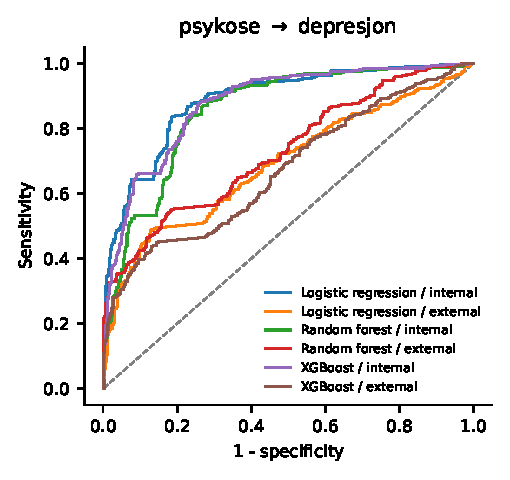
\includegraphics[width=.48\linewidth]{e2_roc_psykose_to_depresjon.pdf}\hfill
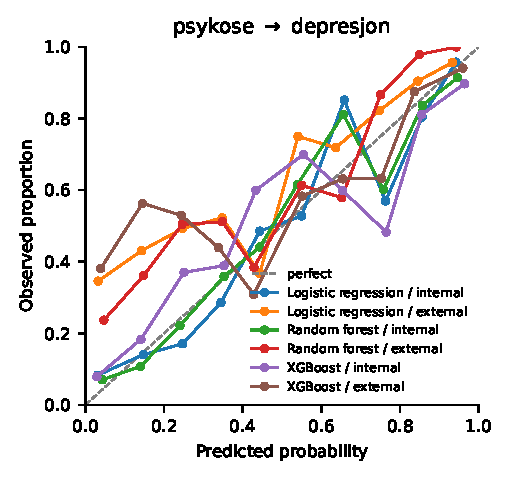
\includegraphics[width=.48\linewidth]{e2_reliability_psykose_to_depresjon.pdf}
\caption{E2, PSYKOSE $\rightarrow$ DEPRESJON. Left: ROC curves of the internal (subject-wise CV on PSYKOSE) and external (frozen model on DEPRESJON) predictions. Right: reliability curves of the same predictions.}\label{fig:e2}\end{figure}
Transfer was asymmetric (Table~\ref{tab:e2}). Models trained on DEPRESJON discriminated
schizophrenia from the held-out controls as well as they had discriminated depression internally
(external AUROC 0.769 to 0.779 versus internal 0.764 to 0.779), because schizophrenia produces the
larger activity deficit. Models trained on PSYKOSE lost 0.13 to 0.21 AUROC when applied to
DEPRESJON (logistic regression 0.885 $\rightarrow$ 0.689; XGBoost 0.877 $\rightarrow$ 0.671), and their
probabilities were both overconfident and shifted: calibration slopes 0.27 to 0.63, intercepts
0.74 to 1.44, Brier 0.22 to 0.29 against 0.25 for the constant prediction (Figure~\ref{fig:e2}).
The label-shift pair DEPRESJON $\rightarrow$ HYPERAKTIV fell to 0.442 to 0.460 with negative slopes.
Subject-level EPV in the training cohorts was 0.6 (DEPRESJON, PSYKOSE after the control split)
and 0.8 (HYPERAKTIV).

\subsection{E3: the calibration blind spot}
% Auto-generated by mlmh.reporting.tables -- do not edit by hand.
\begin{table}[!htbp]
\centering
\caption{E3: calibration alongside discrimination for every model in E1 (subject-wise arm) and E2, plus logistic recalibration of external predictions.}
\label{tab:e3}
\footnotesize
\begin{adjustbox}{max width=\linewidth}
\begin{tabular}{llrrrrr}
\toprule
Exp. & Run & AUROC & Brier & Cal. slope & Cal. intercept & ECE \\
\midrule
E1 & depresjon.logreg.subject\_wise & 0.779 & 0.187 & 0.69 & -0.51 & 0.102 \\
E1 & depresjon.rf.subject\_wise & 0.770 & 0.181 & 0.77 & 0.01 & 0.056 \\
E1 & depresjon.xgboost.subject\_wise & 0.764 & 0.192 & 0.53 & 0.27 & 0.105 \\
E1 & hyperaktiv.logreg.subject\_wise & 0.449 & 0.279 & -0.28 & -0.01 & 0.161 \\
E1 & hyperaktiv.rf.subject\_wise & 0.443 & 0.281 & -0.45 & 0.00 & 0.137 \\
E1 & hyperaktiv.xgboost.subject\_wise & 0.442 & 0.313 & -0.23 & 0.00 & 0.221 \\
E1 & psykose.logreg.subject\_wise & 0.907 & 0.112 & 0.95 & -0.59 & 0.088 \\
E1 & psykose.rf.subject\_wise & 0.893 & 0.115 & 1.03 & -0.12 & 0.052 \\
E1 & psykose.xgboost.subject\_wise & 0.903 & 0.103 & 0.78 & 0.14 & 0.052 \\
E2 & depresjon-to-hyperaktiv.logreg.external & 0.442 & 0.350 & -0.16 & -0.42 & 0.291 \\
E2 & depresjon-to-hyperaktiv.rf.external & 0.461 & 0.317 & -0.15 & 0.33 & 0.214 \\
E2 & depresjon-to-hyperaktiv.xgboost.external & 0.459 & 0.363 & -0.09 & 0.47 & 0.292 \\
E2 & depresjon-to-psykose.logreg.external & 0.779 & 0.193 & 0.50 & 0.06 & 0.079 \\
E2 & depresjon-to-psykose.rf.external & 0.776 & 0.193 & 0.81 & -0.02 & 0.044 \\
E2 & depresjon-to-psykose.xgboost.external & 0.769 & 0.202 & 0.56 & -0.01 & 0.085 \\
E2 & depresjon.logreg.internal & 0.779 & 0.187 & 0.69 & -0.51 & 0.102 \\
E2 & depresjon.rf.internal & 0.770 & 0.181 & 0.77 & 0.01 & 0.056 \\
E2 & depresjon.xgboost.internal & 0.764 & 0.192 & 0.53 & 0.27 & 0.105 \\
E2 & psykose-to-depresjon.logreg.external & 0.689 & 0.262 & 0.27 & 1.20 & 0.202 \\
E2 & psykose-to-depresjon.rf.external & 0.728 & 0.225 & 0.63 & 0.74 & 0.149 \\
E2 & psykose-to-depresjon.xgboost.external & 0.671 & 0.284 & 0.31 & 1.43 & 0.229 \\
E2 & psykose.logreg.internal & 0.885 & 0.137 & 0.77 & -0.10 & 0.061 \\
E2 & psykose.rf.internal & 0.854 & 0.151 & 0.82 & -0.08 & 0.055 \\
E2 & psykose.xgboost.internal & 0.877 & 0.148 & 0.62 & -0.16 & 0.083 \\
E2 & depresjon-to-hyperaktiv.logreg.external+recal & 0.442 & 0.311 & -0.23 & 0.22 & 0.223 \\
E2 & depresjon-to-hyperaktiv.rf.external+recal & 0.461 & 0.301 & -0.20 & 0.37 & 0.176 \\
E2 & depresjon-to-hyperaktiv.xgboost.external+recal & 0.459 & 0.311 & -0.17 & 0.36 & 0.194 \\
E2 & depresjon-to-psykose.logreg.external+recal & 0.779 & 0.211 & 0.72 & 0.56 & 0.139 \\
E2 & depresjon-to-psykose.rf.external+recal & 0.776 & 0.193 & 1.05 & 0.11 & 0.041 \\
E2 & depresjon-to-psykose.xgboost.external+recal & 0.769 & 0.196 & 1.05 & 0.11 & 0.052 \\
E2 & psykose-to-depresjon.logreg.external+recal & 0.689 & 0.254 & 0.35 & 0.99 & 0.185 \\
E2 & psykose-to-depresjon.rf.external+recal & 0.728 & 0.221 & 0.77 & 0.67 & 0.129 \\
E2 & psykose-to-depresjon.xgboost.external+recal & 0.671 & 0.258 & 0.49 & 0.93 & 0.200 \\
\bottomrule
\end{tabular}
\end{adjustbox}
\end{table}

\begin{figure}[!htbp]\centering
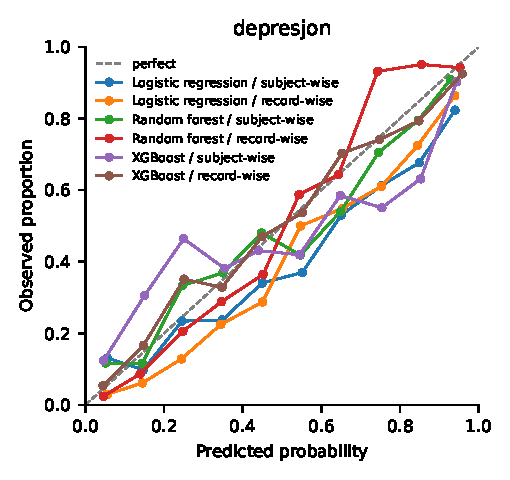
\includegraphics[width=.48\linewidth]{e1_reliability_depresjon.pdf}\hfill
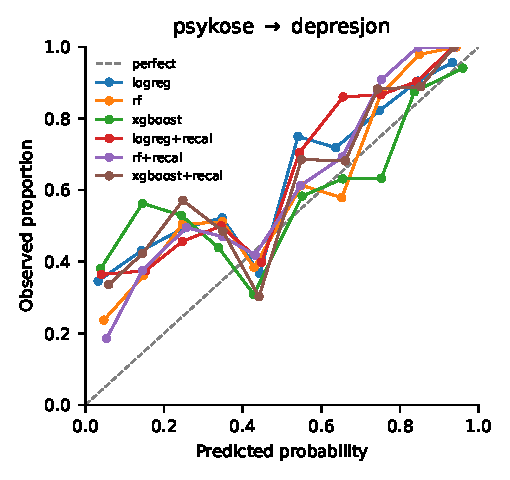
\includegraphics[width=.48\linewidth]{e3_reliability_psykose_to_depresjon.pdf}
\caption{E3. Left: reliability curves of the subject-wise and record-wise E1 models on DEPRESJON. Right: external predictions PSYKOSE $\rightarrow$ DEPRESJON before and after logistic recalibration fitted on the training cohort.}\label{fig:e3}\end{figure}
Under honest internal validation the informative models were already miscalibrated
(Table~\ref{tab:e3}): slopes of 0.53 (XGBoost) to 0.77 (random forest) in DEPRESJON and 0.95
(logistic regression) in PSYKOSE, ECE 0.06 to 0.11 in DEPRESJON, and negative slopes with ECE 0.14
to 0.22 in HYPERAKTIV, where the models had learned nothing but still produced confident
probabilities. Record-wise models were markedly \emph{better} calibrated in-sample, which is
itself a symptom: they were scoring participants they had seen. Recalibrating external predictions
with a slope and intercept fitted on the training cohort's own out-of-fold predictions repaired the
easy direction (DEPRESJON $\rightarrow$ PSYKOSE: slopes 1.05, ECE 0.04 to 0.05 for the ensembles) but
not the hard one (PSYKOSE $\rightarrow$ DEPRESJON: slopes 0.35 to 0.77, ECE 0.13 to 0.20), because the
miscalibration there is a property of the population shift, not of the model.

\subsection{E4: sex-stratified performance}
% Auto-generated by mlmh.reporting.tables -- do not edit by hand.
\begin{table}[!htbp]
\centering
\caption{E4: sex-stratified performance of the subject-wise E1 models (window level, subject-level bootstrap intervals). Subgroups with fewer than six participants or a single class are omitted.}
\label{tab:e4}
\footnotesize
\begin{adjustbox}{max width=\linewidth}
\begin{tabular}{lllllrrr}
\toprule
Cohort & Model & Sex & Participants (cases) & AUROC [95\textbackslash \% CI] & Brier & Cal. slope & ECE \\
\midrule
depresjon & Logistic regression & female & 30 (10) & 0.777 [0.649, 0.872] & 0.182 & 0.75 & 0.120 \\
depresjon & Logistic regression & male & 25 (13) & 0.776 [0.562, 0.882] & 0.192 & 0.62 & 0.091 \\
depresjon & Random forest & female & 30 (10) & 0.763 [0.623, 0.870] & 0.171 & 0.75 & 0.071 \\
depresjon & Random forest & male & 25 (13) & 0.777 [0.626, 0.870] & 0.193 & 0.80 & 0.070 \\
depresjon & XGBoost & female & 30 (10) & 0.755 [0.620, 0.859] & 0.183 & 0.51 & 0.109 \\
depresjon & XGBoost & male & 25 (13) & 0.772 [0.619, 0.868] & 0.203 & 0.55 & 0.120 \\
hyperaktiv & Logistic regression & female & 41 (21) & 0.479 [0.370, 0.602] & 0.275 & -0.10 & 0.152 \\
hyperaktiv & Logistic regression & male & 44 (24) & 0.424 [0.321, 0.543] & 0.283 & -0.49 & 0.168 \\
hyperaktiv & Random forest & female & 41 (21) & 0.491 [0.371, 0.611] & 0.269 & -0.10 & 0.111 \\
hyperaktiv & Random forest & male & 44 (24) & 0.398 [0.278, 0.516] & 0.291 & -0.80 & 0.160 \\
hyperaktiv & XGBoost & female & 41 (21) & 0.498 [0.385, 0.605] & 0.293 & -0.02 & 0.211 \\
hyperaktiv & XGBoost & male & 44 (24) & 0.388 [0.278, 0.505] & 0.332 & -0.44 & 0.230 \\
psykose & Logistic regression & female & 23 (3) & 0.971 [0.915, 0.998] & 0.096 & 1.58 & 0.177 \\
psykose & Logistic regression & male & 31 (19) & 0.890 [0.771, 0.933] & 0.126 & 0.83 & 0.081 \\
psykose & Random forest & female & 23 (3) & 0.966 [0.891, 0.995] & 0.075 & 1.66 & 0.147 \\
psykose & Random forest & male & 31 (19) & 0.874 [0.765, 0.930] & 0.149 & 0.90 & 0.123 \\
psykose & XGBoost & female & 23 (3) & 0.969 [0.904, 0.997] & 0.059 & 1.16 & 0.100 \\
psykose & XGBoost & male & 31 (19) & 0.884 [0.774, 0.933] & 0.140 & 0.71 & 0.121 \\
\bottomrule
\end{tabular}
\end{adjustbox}
\end{table}

Discrimination did not differ materially by sex in DEPRESJON (AUROC 0.76 to 0.78 in both strata)
or HYPERAKTIV (chance in both). In PSYKOSE the female stratum contained three cases, and its
apparently higher AUROC (0.97) rests on those three participants; the intervals overlap the male
stratum's (0.87 to 0.89). Calibration slopes differed more than discrimination between strata
(Table~\ref{tab:e4}).

\subsection{E5: OBF-Psychiatric transdiagnostic and five-class arms}
% Auto-generated by mlmh.reporting.tables -- do not edit by hand.
\begin{table}[!htbp]
\centering
\caption{E5: OBF-Psychiatric (162 participants, single control group). Transdiagnostic binary arm (any psychiatric group vs healthy control; window-level AUROC with subject-level BCa intervals) and five-class arm (macro one-vs-rest AUROC), each under subject-wise and record-wise CV.}
\label{tab:e5}
\footnotesize
\begin{adjustbox}{max width=\linewidth}
\begin{tabular}{lllrrrr}
\toprule
Arm & Model & Split & AUROC / macro-AUROC & Accuracy & Macro-F1 & Cal. slope \\
\midrule
Any psychiatric vs control & Majority class & subject-wise & 0.490 [0.358, 0.614] & 0.641 & 0.391 & 0.25 \\
Any psychiatric vs control & Majority class & record-wise & 0.500 [0.470, 0.529] & 0.641 & 0.391 & 0.25 \\
Any psychiatric vs control & Logistic regression & subject-wise & 0.795 [0.745, 0.848] & 0.741 & 0.725 & 0.78 \\
Any psychiatric vs control & Logistic regression & record-wise & 0.824 [0.777, 0.867] & 0.756 & 0.742 & 0.93 \\
Any psychiatric vs control & Random forest & subject-wise & 0.781 [0.726, 0.837] & 0.739 & 0.705 & 0.75 \\
Any psychiatric vs control & Random forest & record-wise & 0.849 [0.811, 0.887] & 0.782 & 0.755 & 1.07 \\
Any psychiatric vs control & XGBoost & subject-wise & 0.776 [0.729, 0.834] & 0.734 & 0.702 & 0.63 \\
Any psychiatric vs control & XGBoost & record-wise & 0.844 [0.810, 0.885] & 0.781 & 0.755 & 0.90 \\
Five diagnostic groups & Logistic regression & subject-wise & 0.713 [0.677, 0.750] & 0.431 & 0.390 & -- \\
Five diagnostic groups & Logistic regression & record-wise & 0.770 [0.740, 0.799] & 0.484 & 0.444 & -- \\
Five diagnostic groups & Random forest & subject-wise & 0.695 [0.662, 0.735] & 0.434 & 0.350 & -- \\
Five diagnostic groups & Random forest & record-wise & 0.811 [0.786, 0.843] & 0.558 & 0.482 & -- \\
Five diagnostic groups & XGBoost & subject-wise & 0.702 [0.670, 0.743] & 0.448 & 0.355 & -- \\
Five diagnostic groups & XGBoost & record-wise & 0.808 [0.785, 0.842] & 0.558 & 0.467 & -- \\
\bottomrule
\end{tabular}
\end{adjustbox}
\end{table}

In the harmonised 162-participant release, separating any psychiatric group from the healthy
controls reached window-level AUROC 0.776 to 0.795 subject-wise and 0.824 to 0.849 record-wise
(subject level 0.856 to 0.867 versus 0.899 to 0.943). Distinguishing the five diagnostic groups
gave a macro one-vs-rest AUROC of 0.695 to 0.713 (accuracy 0.43 to 0.45 against a 0.28 majority
rate) under subject-wise splitting and 0.770 to 0.811 (accuracy 0.48 to 0.56) under record-wise
splitting (Table~\ref{tab:e5}); the inflation was again largest for the tree ensembles (0.106 to
0.116 in macro-AUROC) and smallest for logistic regression (0.057).

\subsection{Supplementary arm: 1D-CNN on the raw series}
% Auto-generated by mlmh.reporting.tables -- do not edit by hand.
\begin{table}[!htbp]
\centering
\caption{E1, window-level AUROC under subject-wise versus record-wise five-fold cross-validation. Estimates on seed-averaged out-of-fold predictions with subject-level BCa 95\% bootstrap intervals; inflation is the paired record-wise minus subject-wise difference.}
\label{tab:e1_e1_cnn}
\footnotesize
\begin{adjustbox}{max width=\linewidth}
\begin{tabular}{llccc}
\toprule
Cohort & Model & AUROC subject-wise & AUROC record-wise & Inflation (paired) \\
\midrule
depresjon & 1D-CNN & 0.696 [0.576, 0.795] & 0.729 [0.671, 0.784] & 0.033 [-0.063, 0.122] \\
psykose & 1D-CNN & 0.849 [0.744, 0.910] & 0.892 [0.836, 0.935] & 0.043 [-0.000, 0.095] \\
hyperaktiv & 1D-CNN & 0.459 [0.356, 0.588] & 0.513 [0.447, 0.578] & 0.054 [-0.079, 0.189] \\
\bottomrule
\end{tabular}
\end{adjustbox}
\end{table}
% Auto-generated by mlmh.reporting.tables -- do not edit by hand.
\begin{table}[!htbp]
\centering
\caption{E1, participant-level AUROC under subject-wise versus record-wise five-fold cross-validation. Estimates on seed-averaged out-of-fold predictions with subject-level BCa 95\% bootstrap intervals; inflation is the paired record-wise minus subject-wise difference.}
\label{tab:e1subj_e1_cnn}
\footnotesize
\begin{adjustbox}{max width=\linewidth}
\begin{tabular}{llccc}
\toprule
Cohort & Model & AUROC subject-wise & AUROC record-wise & Inflation (paired) \\
\midrule
depresjon & 1D-CNN & 0.738 [0.634, 0.844] & 0.912 [0.837, 0.959] & 0.174 [0.067, 0.270] \\
psykose & 1D-CNN & 0.922 [0.852, 0.976] & 0.986 [0.963, 1.000] & 0.064 [0.016, 0.111] \\
hyperaktiv & 1D-CNN & 0.455 [0.371, 0.563] & 0.529 [0.432, 0.622] & 0.074 [-0.060, 0.208] \\
\bottomrule
\end{tabular}
\end{adjustbox}
\end{table}

A three-block 1D-CNN on the $\log(1+x)$ minute series (30 epochs, five seeds) did not earn its
complexity: under subject-wise splitting its seed-averaged window-level AUROC was 0.696 (95\% CI
0.576 to 0.795) in DEPRESJON, 0.849 (0.744 to 0.910) in PSYKOSE and 0.459 (0.356 to 0.588) in
HYPERAKTIV, below the feature-based models in every cohort, and it was unstable across seeds
(per-seed means 0.61, 0.74 and 0.48). Its window-level inflation under record-wise splitting was
small (0.03 to 0.05, intervals including zero), but at subject level the leaky estimate rose from
0.738 to 0.912 in DEPRESJON (paired difference 0.174, 0.067 to 0.270) and from 0.922 to 0.986 in
PSYKOSE (Table~\ref{tab:e1_e1_cnn}), i.e.\ the network memorised participants rather than days.

\section{Discussion}
\subsection{Principal findings}
Each practice the review found to be common changed conclusions on real data, always towards
optimism. Record-wise splitting added 0.02 to 0.17 AUROC and turned a null result into an apparently
useful classifier. Skipping external validation hid a loss of up to 0.21 AUROC and a collapse of
calibration in one transfer direction while the other direction happened to hold, which is exactly
why one cannot know without doing it. Calibration, never reported for these cohorts, was poor even
under honest validation and was not repairable from the training data alone.

\subsection{Relation to the published benchmarks}
The honest subject-level AUROC of 0.87 to 0.90 on DEPRESJON is consistent with the dataset
authors' leave-one-patient-out baseline \cite{garciaceja2018} and well below the 0.97 to 0.99
that our own record-wise arm produces. Published accuracies above 0.9 on these cohorts
\cite{jmir2025,arxiv2303,psykose_dl2024} are therefore reproducible, but only under the design
that the companion review scores as high risk of bias. The HYPERAKTIV result deserves emphasis:
one day of activity counts carries no information about ADHD versus other psychiatric outpatients
in this sample, and any claim to the contrary that rests on day-level splits should be read as
participant re-identification.

\subsection{Limitations}
Three cohorts from one device family and one country; small participant numbers with wide
subject-level intervals; diagnostic-group labels rather than symptom trajectories; a single window
length; models fixed a priori rather than tuned (tuning inside subject-wise folds would raise honest
performance somewhat but would not change the paired inflation, which is the estimand); no
demographic predictors; and, in E2, a control group split rather than an independent one, because
no independent healthy control actigraphy with the same device is public. The sex analysis in
PSYKOSE is underpowered.

\subsection{Implications}
Authors of ML models on repeated-measures mental-health data should state the unit of splitting,
report subject-level as well as window-level sample sizes and metrics, report calibration slope and
intercept with a reliability curve, and check for shared participants across the datasets they
combine. Reviewers can ask for these in one sentence each. Journals could require them. The
companion review reports how far the field is from that standard; this study reports what the
distance costs.

\section*{Declarations}
Funding: \todo{}. Conflicts of interest: none declared. Ethics: secondary analysis of public,
de-identified data; \todo{institutional determination}. Registration: \todo{OSF}. Data availability:
DEPRESJON, PSYKOSE, HYPERAKTIV and OBF-Psychiatric are available from their authors
\cite{garciaceja2018,jakobsen2020,hicks2021,obf2025}; checksums in the repository. Code
availability: \url{https://github.com/rogerpanel/cv/tree/main/mlmh-appraisal} (\todo{tag; Zenodo DOI}).

\section*{Supplementary material}
S1 TRIPOD+AI checklist (\path{supplement_tripod_checklist.tex}); S2 feature definitions
(\path{src/mlmh/features/actigraphy.py}); S3 per-window predictions and run manifests
(\path{results/real/}).

\begin{thebibliography}{99}\footnotesize
\bibitem{paperA} Ajibola AA, et al. Methodological quality and reporting completeness of machine learning models for mental health prediction: a systematic review and PROBAST+AI / TRIPOD+AI appraisal. \todo{under review / preprint DOI}. 2026.
\bibitem{moons2025} Moons KGM, Damen JAA, Nair T, et al. PROBAST+AI: an updated quality, risk of bias, and applicability assessment tool for prediction models using regression or artificial intelligence methods. BMJ. 2025;388:e082505.
\bibitem{collins2024} Collins GS, Moons KGM, Dhiman P, et al. TRIPOD+AI statement. BMJ. 2024;385:e078378.
\bibitem{garciaceja2018} Garcia-Ceja E, Riegler M, Jakobsen P, et al. Depresjon: a motor activity database of depression episodes in unipolar and bipolar patients. ACM MMSys. 2018. doi:10.1145/3204949.3208125
\bibitem{jakobsen2020} Jakobsen P, Garcia-Ceja E, Stabell LA, et al. PSYKOSE: a motor activity database of patients with schizophrenia. IEEE CBMS. 2020. doi:10.1109/CBMS49503.2020.00064
\bibitem{hicks2021} Hicks SA, Stautland A, Fasmer OB, et al. HYPERAKTIV: an activity dataset from patients with attention-deficit/hyperactivity disorder (ADHD). ACM MMSys. 2021. doi:10.1145/3458305.3478454
\bibitem{obf2025} Garcia-Ceja E, et al. OBF-Psychiatric, a motor activity dataset of patients diagnosed with major depression, schizophrenia, and ADHD. Sci Data. 2025;12. doi:10.1038/s41597-025-04384-3
\bibitem{jmir2025} Explainable AI for depression detection and severity classification from activity data. JMIR Ment Health. 2025;12:e72038.
\bibitem{arxiv2303} Transfer learning for real-time deployment of a screening tool for depression detection using actigraphy. arXiv:2303.07847. 2023.
\bibitem{psykose_dl2024} Unveiling psychotic disorder patterns: a deep learning model analysing motor activity time-series data with explainable AI. Biomed Signal Process Control. 2024; and Objective diagnosis of psychotic disorders using multi-branch deep learning on motor activity signals. Soft Comput. 2024.
\bibitem{vancalster2019} Van Calster B, McLernon DJ, van Smeden M, et al. Calibration: the Achilles heel of predictive analytics. BMC Med. 2019;17:230.
\bibitem{saeb2017} Saeb S, Lonini L, Jayaraman A, Mohr DC, Kording KP. The need to approximate the use-case in clinical machine learning. GigaScience. 2017;6:gix019.
\end{thebibliography}
\end{document}
